% !TEX root=../master.tex
\chapter{GPS-Denied Self-Pose Estimation}
\label{ch:self_pose}

A fundamental component of performing a target handoff without GPS is accurate estimation of the self-pose of each vehicle.
Without GPS, there is no global frame of reference that is common between the two vehicles. 
Accordingly, all information shared about the target must be coordinated using relative transformations. 
These relative transformations depend heavily upon each vehicle's estimate of its self-pose as well. 
Small errors in self-pose estimates are amplified by long distances and can lead to large errors in the estimated relative transformation between the two vehicles. 
This chapter will discuss methods for estimating the self-pose, followed by a discussion of estimating the relative-pose in Chapter~\ref{ch:relative_pose}. 
Both chapters are focused on estimation for fixed wing UAV in GPS-denied environments.

\section{Background}
There has been extensive work done on estimating the attitude of a fixed-wing aircraft both using non-linear~\cite{Mahony11} and linear~\cite{LiuZhouFu08} methods.
For this work we estimate the attitude state of the filter using a complimentary filter on SO(3), based upon the work done in \cite{Mahony11}. 
While the filter approach and algorithm remain the same, we do make a slight extension to the filter presented by Mahony et al. to better account for variability in the magnitude of the airspeed. The details of the filter, as well as our extension, will be discussed below.


% Two of these methods are discussed and compared here in an effort to identify which method provides the most accurate results for GPS-free fixed-wing estimation. In addition to making comparisons between existing filters, some improvements are proposed which extend previous work. First, a multiplicative extended Kalman filter (MEKF) for fixed-wing attitude estimation will be discussed, followed by an explanation of a non-linear complimentary filter which extend the work done in \cite{Mahony11}.
% % \section{Multiplicative Extended Kalman Filter}
%
% \subsection{Introduction}
% A common method of estimating fixed-wing attitude is by using an extended Kalman filter (EKF) to estimate the roll, pitch, and yaw of the aircraft. The main deficiencies of this approach are that (1) Euler angles contain a singularity when pitch is $\pm 90^{\degree}$ and (2) the repeated use of trigonometric functions can be computationally expensive.
% The multiplicative extended Kalman filter (MEKF) uses a quaternion, rather than Euler angles, to propagate the attitude state, eliminating the singularity and allowing for computationally efficient update and propagation steps. In order to propagate the attitude on $SO(3)$ the quaternion multiply operator must be used, hence the name "multiplicative extended Kalman filter." Because the quaternion is an over-parameterized representation of roll, pitch, and yaw, we cannot define a meaningful covariance for each of the four elements in the quaternion. Instead, we define the error covariance about the minimal representation, or error state, and perform the update using this error state. The covariance matrix, $\P$, is defined about the error state, which is one less in dimensionality than the full state vector. We must also derive error state versions of the propagation and measurement Jacobians in order to appropriately use the error state to update the estimates.
%
% Architecturally, the MEKF is very similar to the EKF. The primary difference is that because the covariance matrix is defined with respect to the error state, the update step outputs $\dx$, the error state, rather than producing $\x[\hat]$, as in the case of the EKF. Figures \ref{fig:ekf_diagram} and \ref{fig:mekf_diagram} show the respective high-level architectures of the EKF and the MEKF.
% \begin{figure}
% 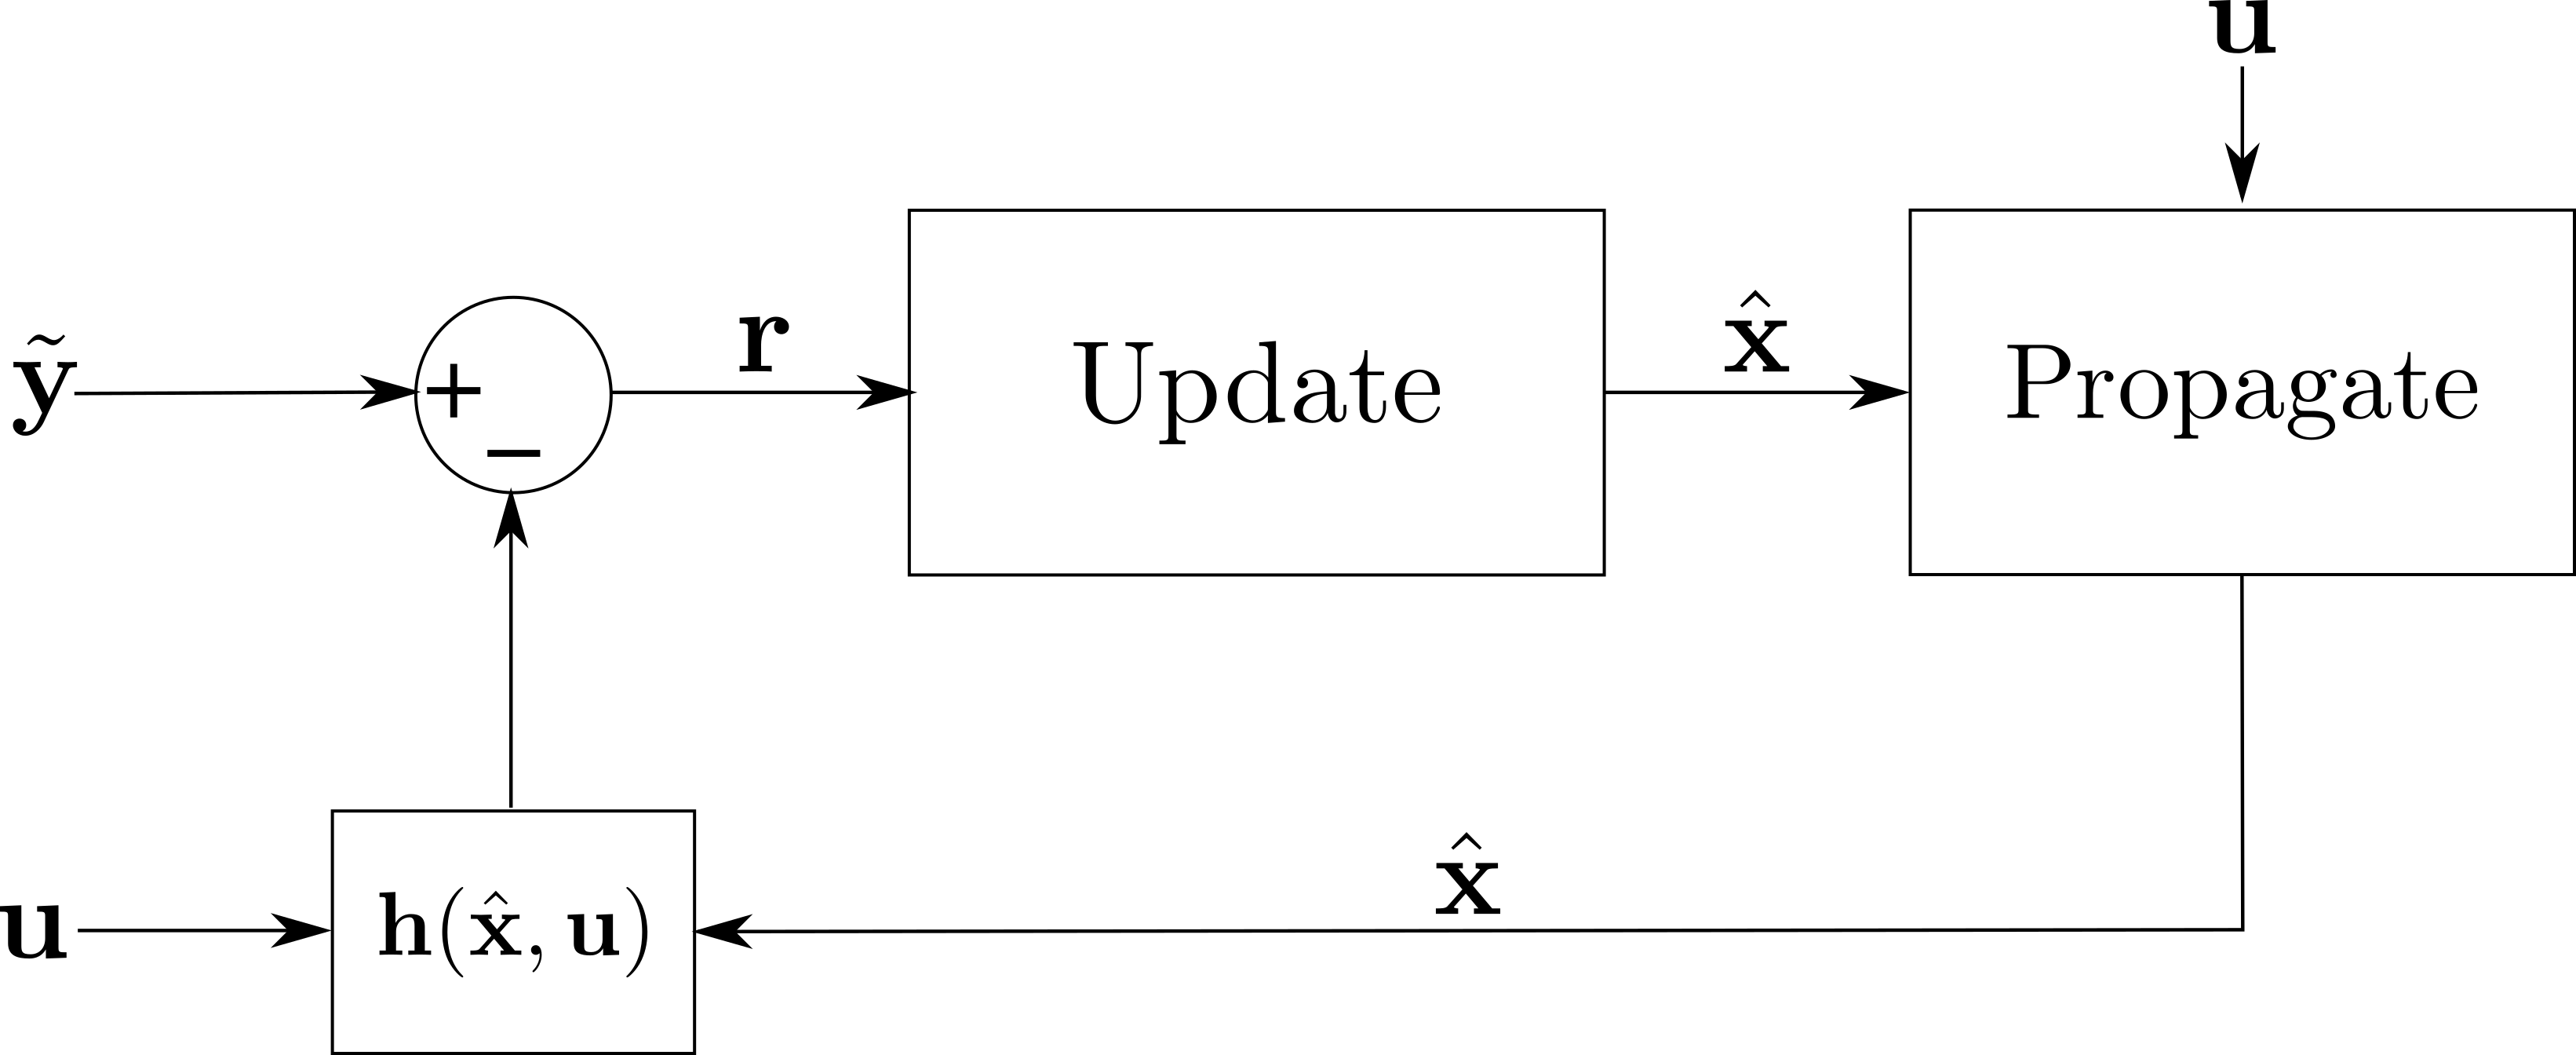
\includegraphics[width=\columnwidth]{figures/ekf_diagram.png}
% \caption{EKF flow diagram}
% \label{fig:ekf_diagram}
% \end{figure}
%
% \begin{figure}
% 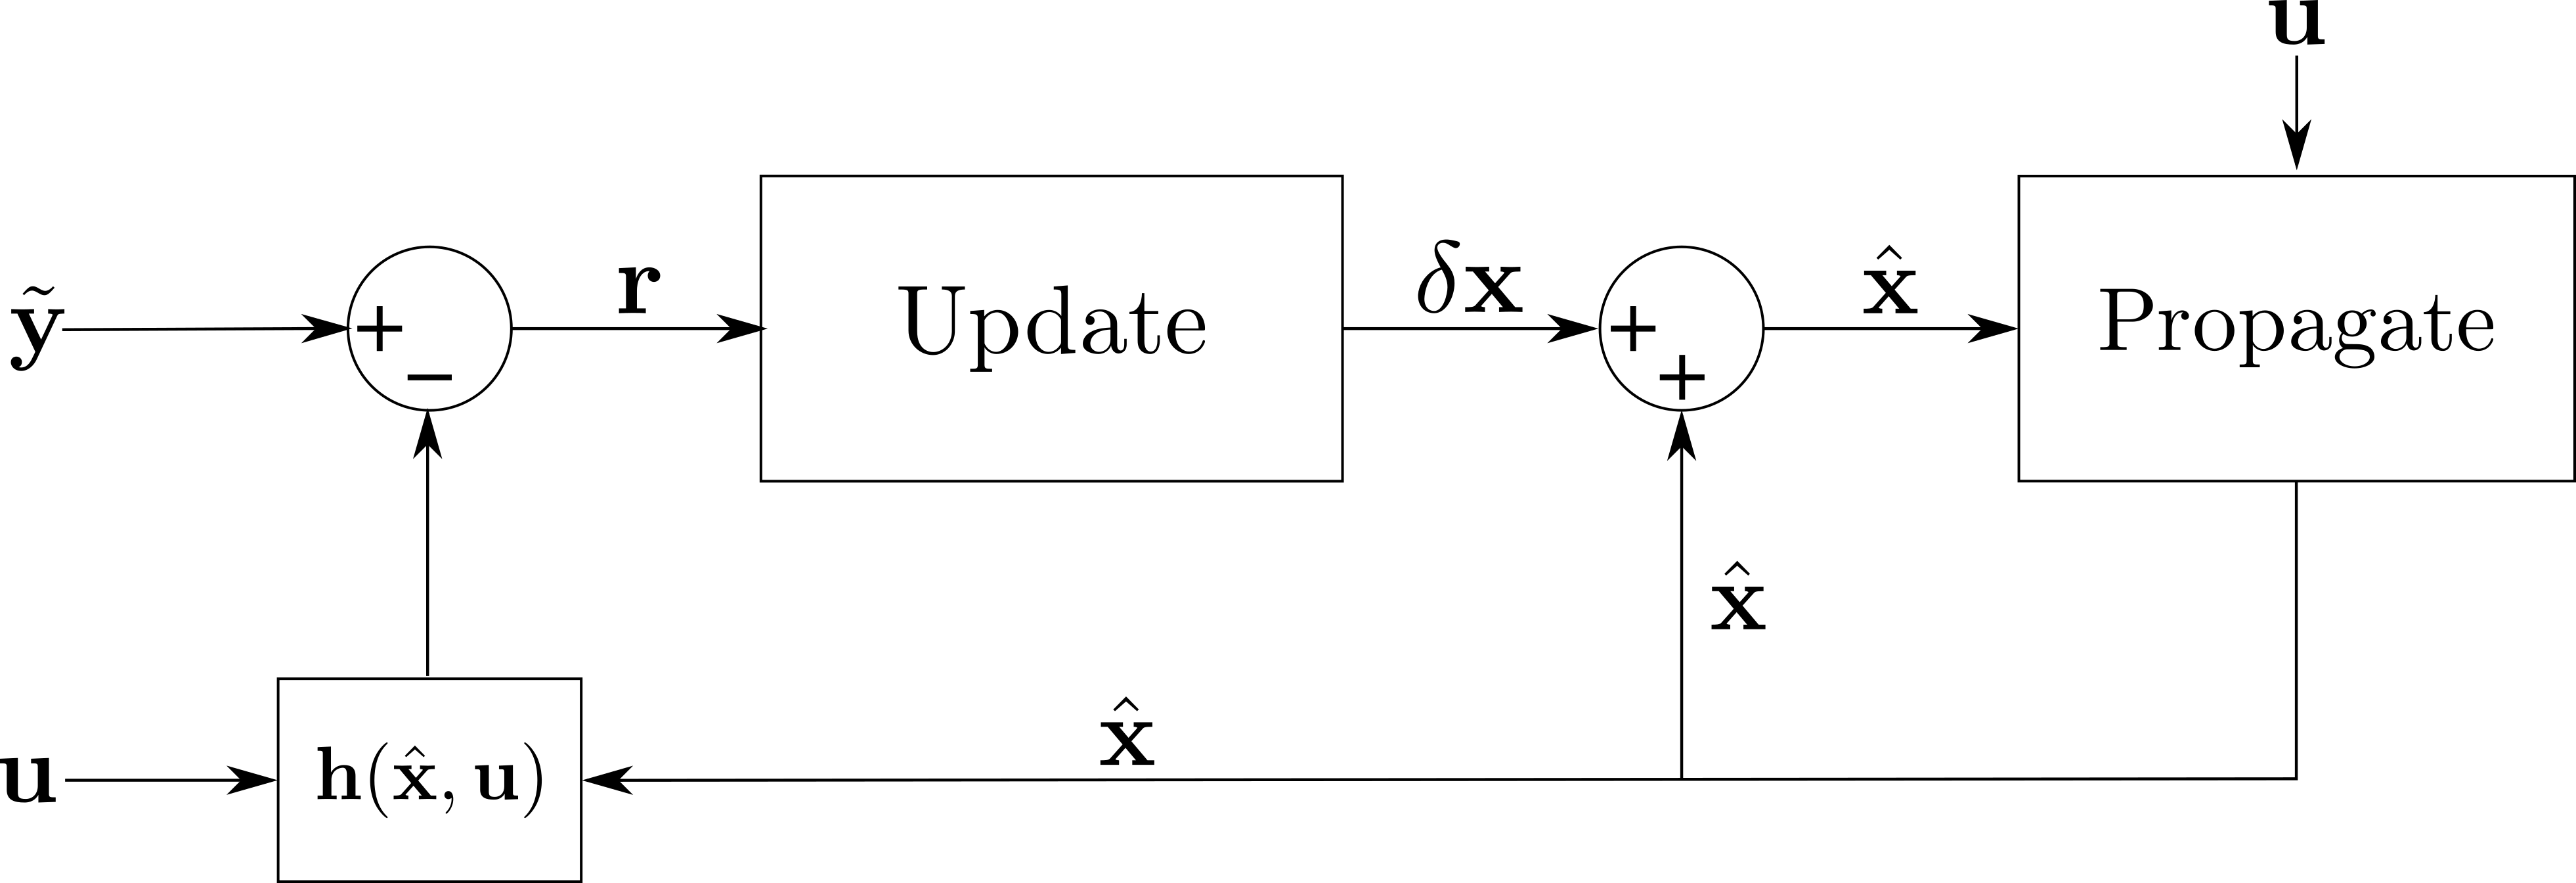
\includegraphics[width=\columnwidth]{figures/mekf_diagram.png}
% \caption{MEKF flow diagram}
% \label{fig:mekf_diagram}
% \end{figure}
%
% The MEKF presented here draws heavily from \cite{RMEKF}, but also offers some unique contributions. This implementation focuses specifically on fixed-wing aircraft and makes some improvements based on the dynamics specific to fixed-wing vehicles. For example, the filter concurrently estimates the airspeed vector using an estimate of the angle of attack along with estimating gyro biases to improve the attitude estimates. The filter also estimates the attitude independent of GPS data.
%
%
% \subsection{Quaternions}
% Before describing the core implementation of the filter, it is important to have a basic understanding of quaternions and their properties.
% This section provides an overview of the quaternion operations and conventions used in this implementation. This section is intended to be used as a useful reference, especially for the implementation of the filter. It is not, however, a comprehensive guide to quaternions and does not provide the full derivation for most of the equations used. For a more in-depth resource on quaternions, we refer the reader to \cite{eq:MEKF},~\cite{Trawny05}.
% \label{sec:quaternions}
%
%
% \subsubsection{Definitions}
%
% Quaternions are a hyper-complex four-dimensional representation of attitudes and rotations. We can define a quaternion, generally as
% % %%
% % \comment{REVIEW: Does this need to be vector or scalar notation}
% % %%
% \begin{equation}
% \q = \qw + q_x \ii + q_y \jj + q_z \kk \;
% \end{equation}
% where $\q \in \mathbb{H}$.

% Quaternions can be represented in multiple ways, each resulting in slightly different version of the basic definitions and operations used. This section will describe the conventions used for all quaternion variables and operations throughout the paper.

% Specifically, we will be using the Hamiltonian definition of a quaternion, as opposed to JPL notation (\cite{JPL}). The Hamiltonian definition of a quaternion is given by
% \begin{align} \label{eq:complex_products}
% \begin{split}
% \ii \jj = -\jj \ii &= \kk \;, \\
% \jj \kk = -\kk \jj &= \ii \;, \\
% \kk \ii = -\ii \kk &= \jj \;, \\
% \ii^2 = \jj^2 = \kk^2 = \ii \jj \kk &= -1 \;.
% \end{split}
% \end{align}

% For convenience, we will define the quaternions as
% \begin{equation}
%   \label{eq:q_definition}
%   \q = \begin{bmatrix} \qvec \\ \qw \end{bmatrix} \;,
% \end{equation}
% where $\qvec$ is the vector component, representing the axis of rotation, and $\qw$ is the scalar component, representing the magnitude of rotation. The vector portion, $\qvec$, is defined as
% \begin{equation}
%   \label{eq:qvec}
% 	\qvec=\begin{bmatrix} q_x & q_y & q_z \end{bmatrix}^\transpose \;.
% \end{equation}


% \subsubsection{Quaternion multiplication}

% Quaternions have no defined addition or subtraction operators. Instead the quaternion multiplication operator is used to combine quaternions. The Hamiltonian quaternion multiply is defined according to
% \begin{align} \label{eq:q_mult}
% \p \otimes \q &=
%     \begin{bmatrix}
%     \pw \I + \skewmat{\pvec} & \pvec \\
%     -\pvec^\transpose & \pw
%     \end{bmatrix}
%     \begin{bmatrix} \qvec \\ \qw \end{bmatrix}\; \\
% &= \begin{bmatrix}
%     \qw \I - \skewmat{\qvec} & \qvec \\
%     -\qvec^\transpose & \qw \end{bmatrix}
%     \begin{bmatrix} \pvec \\ \pw \end{bmatrix}\;.
% \end{align}
% Also note that $\skewmat{\cdot}$ defines the skew-symmetric operator, such that
% \begin{equation} \label{eq:skewmat_def}
% \skewmat{\vect{a}} \triangleq \begin{bmatrix}
% 0 & -a_z & a_y \\
% a_z & 0 & -a_x \\
% -a_y & a_x & 0 \end{bmatrix}.
% \end{equation}


% \subsubsection{Error state}

% We can define the true attitude quaternion state as
% \begin{equation} \label{eq:q_actual}
% \q = \q[\hat] \otimes \dq
% \end{equation}
% where $\q[\hat]$ is the estimated attitude and $\dq$ is the error in the attitude.
% Solving for $\dq$ in \eqref{eq:q_actual}, we get
% \begin{equation}
% \dq = \q[\hat]^{-1} \otimes \q \;.
% \end{equation}
% As previously mentioned, we cannot define a covariance about a quaternion, so we use a minimal representation of the quaternion error, denoted by $\dth$ such that
% \begin{equation} \label{eq:dq}
% \dq = \exp\left(\half \dth\right) \;
% \end{equation}
% where $\exp(\cdot)$ is defined by \eqref{eq:quat_exp}.
% When $\dq[\bar]$ is small, we can use a first order approximation of \eqref{eq:dq},
% \begin{equation}
% \dq = \begin{bmatrix} \half \dth \\ 1 \end{bmatrix},
% \end{equation}
% which leads to
% \begin{equation}
% \dth = 2\dq[\bar] \;.
% \end{equation}

% \subsubsection{Exponential mapping}

% In order to map the error state vector, $\dth$, which is a minimal representation in $\mathbb{R}^3$, to the quaternion in $SO(3)$, we use an exponential mapping, defined as
% \begin{equation} \label{eq:quat_exp}
%   \exp(\delta) \triangleq \begin{bmatrix} \sin\norm{\delta}\frac{\delta}{\norm{\delta}} \\ \cos\norm{\delta} \end{bmatrix}\;.
% \end{equation}
% It is important to note that as $\norm{\delta} \approaches 0$, the exponential mapping becomes numerically unstable. Therefore, when $\norm{\delta}$ is sufficiently small, we can approximate the exponential mapping by using its limit, given by
% \begin{equation} \label{eq:exp_lim}
% \lim_{\norm{\delta}\approaches 0}\exp(\delta) = \begin{bmatrix} \delta \\ 1 \end{bmatrix}\;.
% \end{equation}

% The exponential mapping, in combination with the $\otimes$ operator, allows us to update the quaternion by some minimal representation error state, $\dth$, while still remaining completely on the $SO(3)$ manifold. This is performed according to
% \begin{equation} \label{eq:q_update}
% \q^+ = \q^- \otimes \exp\left(\half\dth\right) \;.
% \end{equation}
% Or, when $\norm{\dth}$ is small, we use the limit of the exponential, given in \eqref{eq:exp_lim}, resulting in
% \begin{equation}
% \q^+ = \q^- \otimes \begin{bmatrix} \half\dth \\ 1 \end{bmatrix} \;.
% \end{equation}
% % Commonly, linear approximations of this mapping are used and then normalized back to the manifold, but using this exponential mapping allows us to remain on the manifold and minimize linearization errors.

% In some recent literature (\cite{boxplus_herztberg}), the combination of using quaternion multiplication and the exponential mapping in order to update a quaternion is also referred to as the ''boxplus'' operator ($\boxplus$). For example, equation \eqref{eq:q_update} could be written as
% \begin{equation}
% \q^+ = \q^- \boxplus \dth
% \end{equation}
% using boxplus notation.
% While the two operations are synonymous, we will use the notation in equation \eqref{eq:q_update} for verbosity.


% \subsubsection{Rotations}

% It is also often necessary to produce a rotation matrix from the quaternion attitude state. In this paper, quaternion rotation matrices are computed according to
% \begin{equation} \label{eq:Rq}
%   \R(\q) = \qw^2 \I - 2\qw \skewmat{\qvec} + \qvec\qvec^\transpose + \skewmat{\qvec}^2 \;.
% \end{equation}
% It is also possible to represent $\skewmat{\qvec}^2$ as
% \begin{equation}
% \skewmat{\qvec}^2 = \qvec \qvec^\transpose - (1 - \qw^2)\I \;
% \end{equation}
% and rewrite \eqref{eq:Rq} as
% \begin{equation}
% \R(\q) = (2\qw^2 - 1)\I - 2\qw\skewmat{\qvec} + 2\qvec\qvec^\transpose \;.
% \end{equation}


% \subsubsection{Time derivative}

% In this implementation of the MEKF, the first order quaternion derivative is used, given by
% \begin{equation} \label{eq:qhatdot}
%   \q[\hatdot] = \half \q[\hat] \otimes \begin{bmatrix} \angvel[\hat] \\ 0 \end{bmatrix} \;.
% \end{equation}
% This can also be expressed as
% \begin{equation}
% \q[\hatdot] = \half \Omega(\angvel[\hat]) \q[\hat]
% \end{equation}
% where
% \begin{equation} \label{eq:Omega}
%   \bOmega(\angvel) = \begin{bmatrix} 0 & \omega_z & -\omega_y & \omega_x \\
%                                       -\omega_z & 0 & \omega_x & \omega_y \\
%                                       \omega_y & -\omega_x & 0 & \omega_z \\
%                                       -\omega_x & -\omega_y & -\omega_z & 0 \end{bmatrix} \;.
% \end{equation}


% \subsubsection{Time integration}

% Quaternion integration is primarily based upon trying to perform some incremental update,
% \begin{equation}
% \q_{t + \Delta t} = \q_t \otimes \q_{\Delta t}.
% \end{equation}
% Zero-th order integration assumes a constant nominal angular velocity, $\angvel_0$, and is given by
% \begin{equation}
% \q_{t + \Delta t} = \q_t + \Delta t \left(\half \q_t \otimes \begin{bmatrix} \angvel_0 \\ 0 \end{bmatrix} \right) \;.
% \end{equation}
% Note that this form of quaternion integration will depart slightly from the $SO(3)$ manifold, so the quaternion must be manually normalized back onto the manifold.
% A first order quaternion integrator is used to propagate the quaternion estimate, which assumes that angular velocity is evolving linearly between integration steps.
% The integration, as derived in \cite{Trawny05}, is given by
% \begin{equation} \label{eq:q_int}
% % \small
%   \q(t_{k+1}) = \Bigg[ \matexp\left(\half \bOmega(\bar{\angvel})\Delta t \right) + \frac{1}{48} \bigg( \bOmega\big( \angvel( t_{k+1})\big) \bOmega\big( \angvel(t_k)\big) - \bOmega\big( \angvel( t_{k})\big) \bOmega\big( \angvel(t_{k+1})\big)\bigg) \Delta t^2 \Bigg] \q(t_k)
% \end{equation}
% where $\matexp\left(A\right)$ is the matrix exponential,
% $\Omega(\angvel)$ is given by \eqref{eq:Omega}, and
% \begin{equation}
%   \bar{\angvel} = \frac{\angvel(t_{k+1}) + \angvel(t_k)}{2} \;.
% \end{equation}

% % \subsection{Euler angle/quaternion relationship}
% \subsubsection{Euler angle decomposition}

% It is often useful to be able to convert between Euler angle and quaternion representations of the attitude.
% % Quaternion to euler
% For a given quaternion,
% $$ \q = \begin{bmatrix} q_x \\ q_y \\ q_z \\ \qw \end{bmatrix} \;, $$
% the corresponding roll ($\phi$), pitch ($\theta$), and yaw ($\psi$) are given by
% \begin{align}
% \phi &= \text{atan}\left(\frac{2 \qw q_x + 2 q_y q_z}{q_z^2 - q_x^2 - q_y^2 + \qw^2}\right) \;, \\
% \theta &= \text{asin}\left(2 \qw q_y - 2 q_x q_z\right) \;, \\
% \psi &= \text{atan}\left(\frac{2 \qw q_z + 2 q_x q_y}{q_x^2 - q_y^2 - q_z^2 + \qw^2}\right) \;. \label{eq:quat_psi}
% \end{align}
% % Euler to Quaternion
% Conversely, for a given set of Euler angles, the corresponding quaternion can be constructed according to
% \begin{align}
% q_x &= \cos\frac{\psi}{2} \cos\frac{\theta}{2} \sin\frac{\phi}{2} - \sin\frac{\psi}{2} \sin\frac{\theta}{2} \cos\frac{\phi}{2} \;, \\
% q_y &= \cos\frac{\psi}{2} \sin\frac{\theta}{2} \cos\frac{\phi}{2} + \sin\frac{\psi}{2} \cos\frac{\theta}{2} \sin\frac{\phi}{2} \;, \\
% q_z &= \sin\frac{\psi}{2} \cos\frac{\theta}{2} \cos\frac{\phi}{2} - \cos\frac{\psi}{2} \sin\frac{\theta}{2} \sin\frac{\phi}{2} \;, \\
% \qw &= \cos\frac{\psi}{2} \cos\frac{\theta}{2} \cos\frac{\phi}{2} + \sin\frac{\psi}{2} \sin\frac{\theta}{2} \sin\frac{\phi}{2} \;.
% \end{align}


% %%%%%%%%%%%%%%%%%%%%%%%%%%%%%%%%%%%%%%%%%%%%%%%%%%%%%%%%%%%%%%%%%%%%%%%
% %%%%%%%%%%%%%%%%%%%%%%%% FILTER IMPLEMENTATION %%%%%%%%%%%%%%%%%%%%%%%%
% %%%%%%%%%%%%%%%%%%%%%%%%%%%%%%%%%%%%%%%%%%%%%%%%%%%%%%%%%%%%%%%%%%%%%%%
% \vspace{2em}
% \subsection{Filter Implementation}
% \label{sec:implemenation}
% Many of the equations used here are based upon the MEKF framework given in~\cite{RMEKF}. This section will seek to show derivations for novel changes to the basic MEKF implementation and other additions which are specific to a fixed-wing model, but we refer the reader to other MEKF literature for in depth derivations of the basic filter framework (\stcomment{cite key MEKF papers here}).\\

% %%%%%%%%%%%%%%%%%%%%%%%%%%%%% DEFINITIONS %%%%%%%%%%%%%%%%%%%%%%%%%%%%%
% \subsubsection{Definitions}

% The MEKF implemented here primarily seeks to accurately estimate the attitude quaternion, but the state also includes gyro bias and angle of attack to help improve the estimator's accuracy.
% The state is defined as
% \begin{equation}
%     \x = \begin{bmatrix} \q \\ \gbias \\ \alpha \end{bmatrix}
% \end{equation}
% where $\q$ is the attitude quaternion, $\gbias$ represents the gyro biases along the x, y, and z axes, and $\alpha$ is the vehicle's angle of attack.

% % [ST] TODO: with the airspeed in the input, do we need to add airspeed noise throughout and adjust our jacobians?
% The input vector is composed of the gyro and airspeed sensor measurements and is given by
% $$ \u = \begin{bmatrix} \tilde{\angvel} \\ v_a \end{bmatrix}, $$
% where
% $$ \tilde{\angvel} = \begin{bmatrix} \tilde{\omega}_x \\ \tilde{\omega}_y \\ \tilde{\omega}_z \end{bmatrix}.  $$
% and $v_a$ is the airspeed.
% We define our measurement as the accelerometer sensor data, $\accel[\tilde]$, and the heading measurement extracted from the magnetometer, $\tilde{\psi}$, according to
% $$ \y = \begin{bmatrix} \tilde{\accel} \\ \tilde{\psi} \end{bmatrix} =
%         \begin{bmatrix} \tilde{a}_x & \tilde{a}_y & \tilde{a}_z & \tilde{\psi} \end{bmatrix}^{\transpose} \;.$$

% The heading information can be determined from the magnetometer data, $\magnet$, by
% rotating the sensor data into the vehicle 1 (unpitched, unrolled) frame, isolating the heading angle, and factoring in the magnetic field declination, $\magdec$, according to
% \begin{subequations} \label{eq:mag2heading}
% \begin{align}
%   \magnet^{v1} &= \Rot{b}{v1}\magnet \\
%   % [ST] TODO: check for other atan2 implementations
%   \psimag &= \atantwo(\magnet^{v1}_{y}, \magnet^{v1}_{x}) \\
%    \tilde{\psi} &= \magdec - \psimag \;.
% \end{align}
% \end{subequations}
% The value of $\magdec$ can be predetermined based upon the approximate latitude and longitude at which the aircraft will be flown.
% Figure~\ref{fig:magnetometer} gives a geometrical representation of the magnetometer-based heading measurement.
% \begin{figure}[hbt]
%   \centering
%   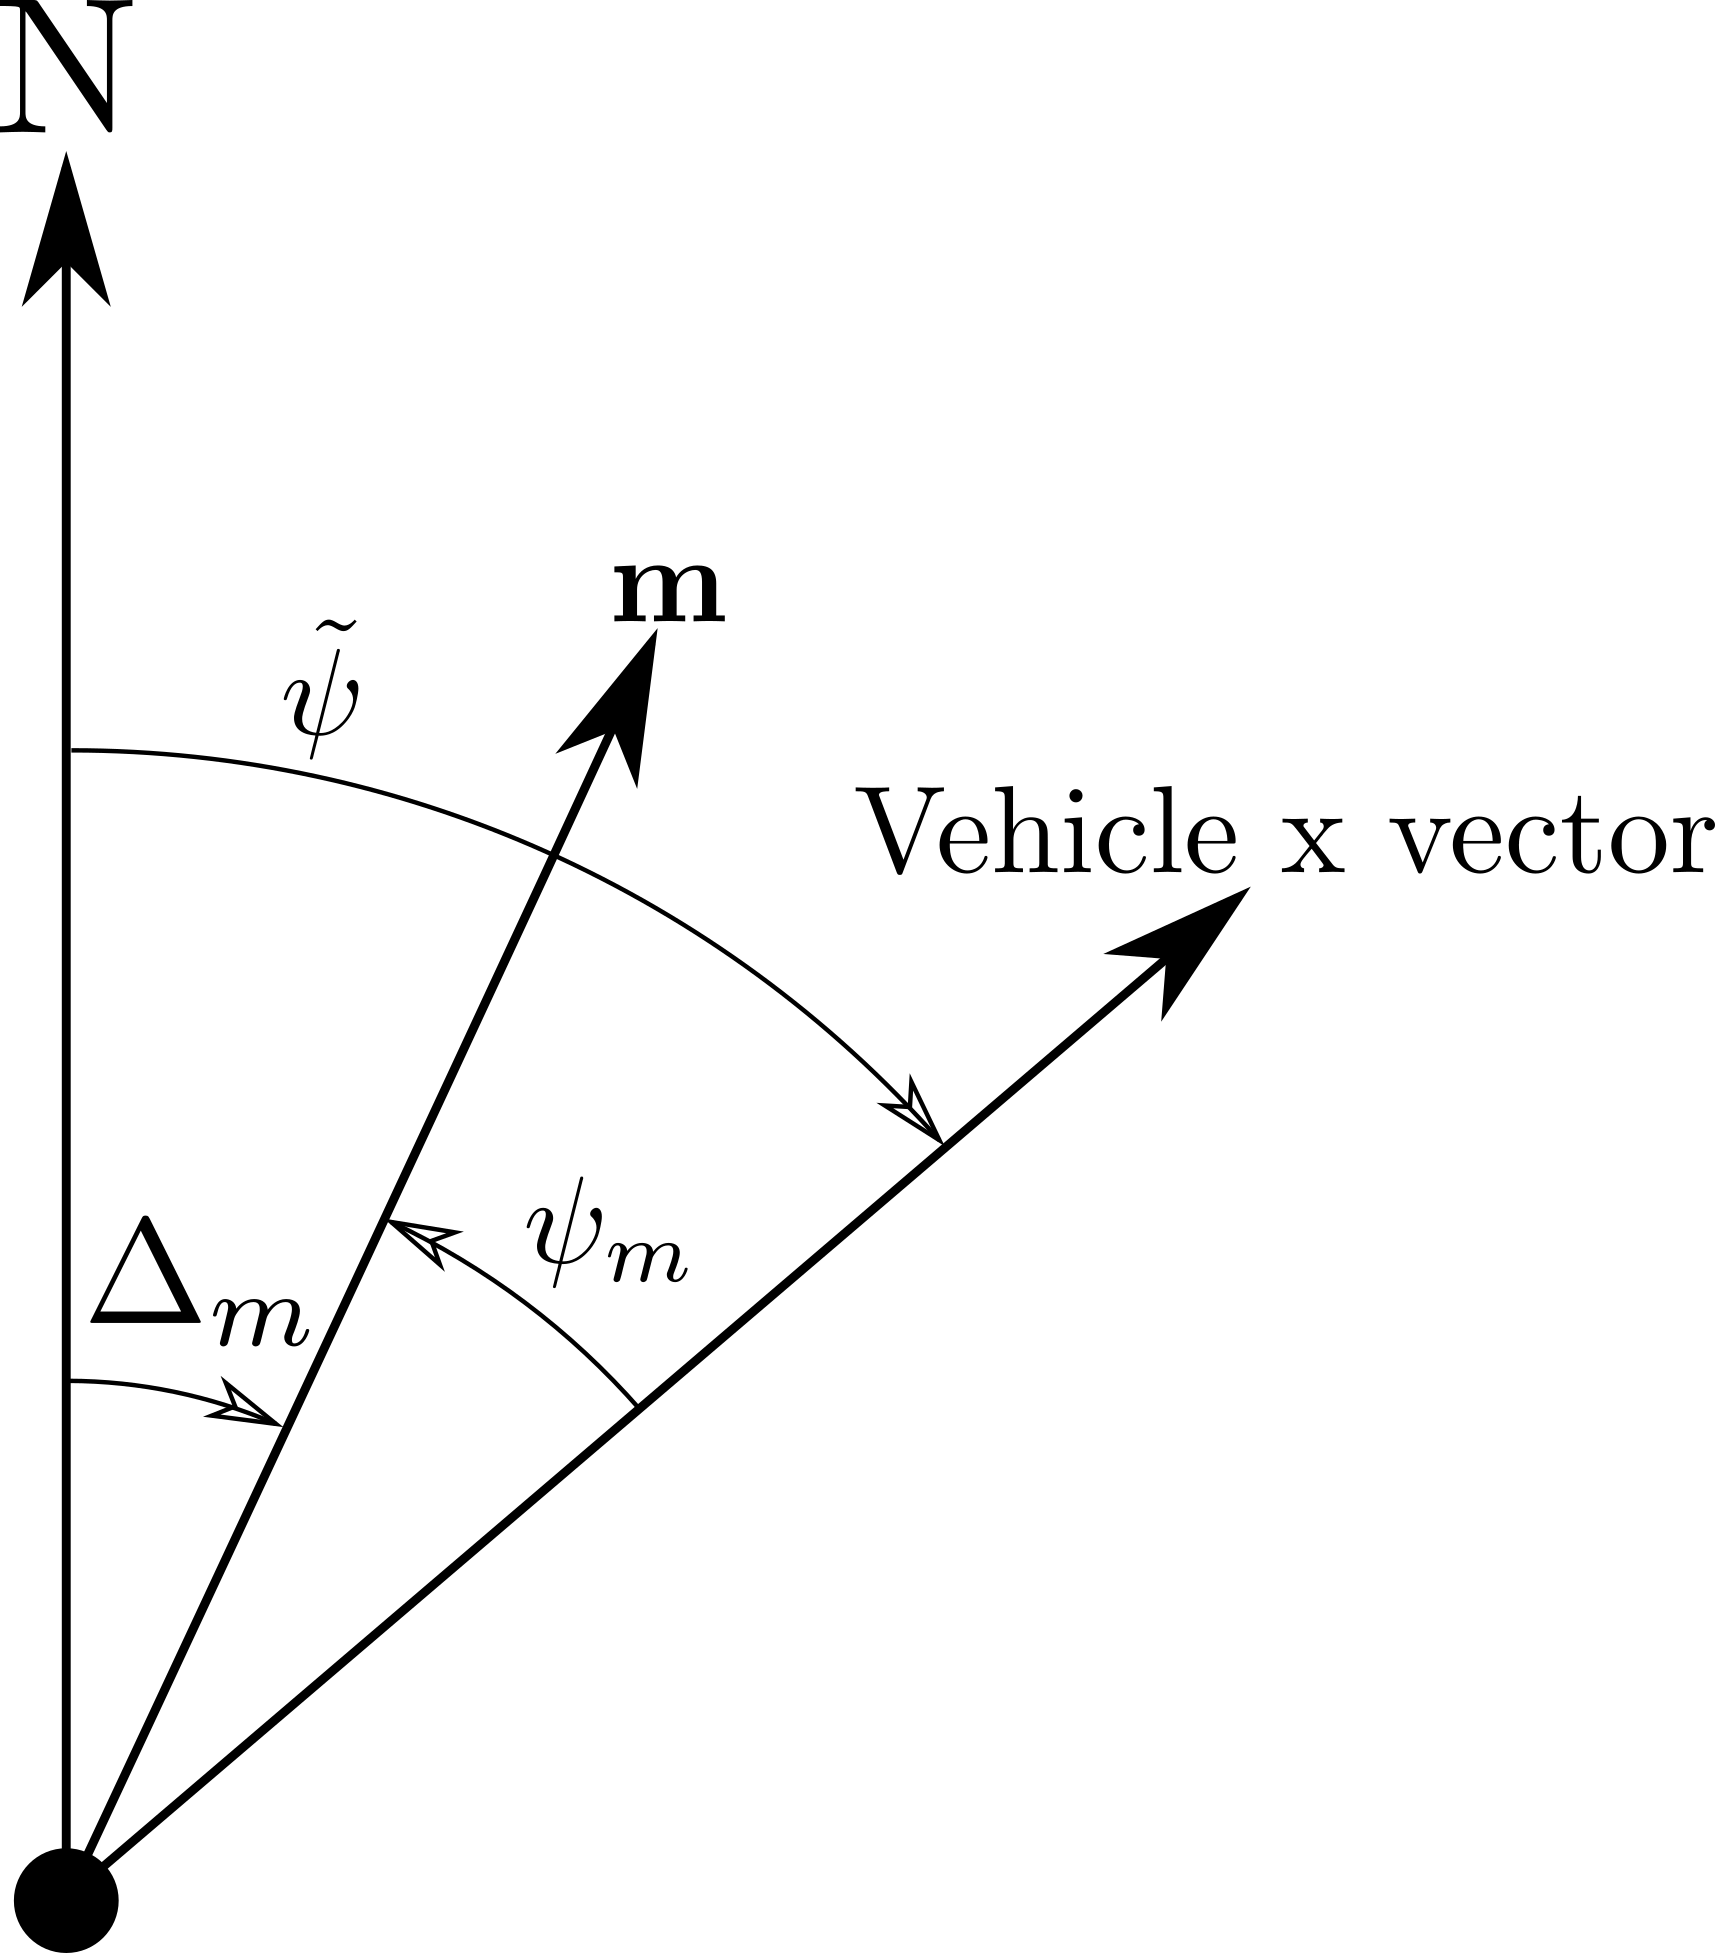
\includegraphics{figures/mekf_mag_geom}
%   \caption{XY-plane representation of heading measurement from magnetometer sensor reading.}
%   \label{fig:magnetometer}
% \end{figure}
% \newline

% %%%%%%%%%%%%%%%%%%%%%%%%%%%%% PROPAGATION %%%%%%%%%%%%%%%%%%%%%%%%%%%%%
% \subsubsection{State propagation}
% The state propagation dynamics are denoted by
% \begin{equation} \label{eq:estimator_dynamics}
%  \x[\hatdot] = \f(\x[\hat], \u) \;.
% \end{equation}
% However, because the not all of the dynamics are linear, the propagation step is best expressed in terms of the individual state components.

% The dynamics of a quaternion are often defined according to the first order time derivative in \eqref{eq:qhatdot} as
% \begin{equation*}
% \q[\hatdot] = \half \q[\hat] \otimes \begin{bmatrix} \angvel[\hat] \\ 0 \end{bmatrix} \;.
% \end{equation*}
% However, in practice, we will use the first order quaternion integrator given in \eqref{eq:q_int}.

% We assume the gyro bias is relatively constant, with some noise and slow, unpredictable drift, so we define the bias dynamics according to
% \begin{equation} \label{eq:gbias_dynamics}
%   \gbias[\hatdot] = \vect{0} \;.
% \end{equation}

% The estimated angle of attack is propagated according to a linearized dynamic model, adapted from the model used in \cite{Mahony11}, given by
% \begin{equation}
%   \hatdot{\alpha} = -\frac{c_0(v_a)}{v_a}\hat{\alpha} + \dot{\theta} + (\alpha_0(v_a))
% \end{equation}
% where
% \begin{equation} \label{eq:c0_Va}
% c_0(v_a) = \frac{k_\delta - k_T v_a^2}{m}
% \end{equation}
% and
% \begin{equation}
% \alpha_0(v_a) = \frac{g}{v_a} - \frac{k_L}{m}v_a \;.
% \end{equation}
% The function $c_0(v_a)$ represents the effects of the thrust force and $\alpha_0(v_a)$ acts as a set point needed to maintain level flight, based on airspeed and the lift force.
% In \cite{Mahony11}, $c_0$ and $\alpha_0$ are constants, but we have replaced them with simple functions of airspeed in order to maintain greater model accuracy across varying speeds. The derivation for this adaptation is given in Appendix \ref{append:alpha_derivation}.

% For our implementation we achieved fairly good estimation of $\alpha$ using the following values for our constants:
% %%
% % \todo[inline]{Update or remove these constants}
% %%
% \begin{align*}
%   k_\delta &= 40 \\
%   k_T &= -4.07 \\
%   k_L &= 0.245 \\
%   m &= 3.92\text{ kg} \;.
% \end{align*}
% These values are system dependent and can be obtained experimentally.

% Because the covariance matrix represents the spread of the error state, in order to compute the propagation Jacobians, we need to derive an error state measurement model, $\bar{\f}$, given by
% \begin{subequations} \label{eq:dxdot_error}
% \begin{align}
% \dx[\dot] &= \f[\bar](\dx,\noiseu,\x[\hat],\u) + \noise \;. \\
% 		&= \f(\x, \u + \noiseu) - \f(\x[\hat], \u) \\
%         &= \f(\x[\hat] + \dx, \u + \noiseu) - \f(\x[\hat], \u) \;.
% \end{align}
% \end{subequations}
% %%
% % \todo[inline]{Add derivations here}
% %%
% The first-order approximation of the error-state dynamics are
% %\begin{subequations}
% \begin{align}
%   \label{eq:error_dynamics_dth}
%   \dth[\dot] &\approx -\skewmat{\angvel[\tilde] - \gbias[\hat]}\dth - \dgbias - \noiseu_{\angvel} \\
%   \label{eq:error_dynamics_dgbias}
%   \dgbias[\dot] &= \noise_{\gbias} \\
%   \label{eq:error_dynamics_dalpha}
%   \dot{\dalpha} &= \frac{-(k_\delta - k_T v_a^2)}{mv_a}\dalpha - (\dgbias + \noiseu_{\angvel})\cdot\vect{e}_2 \;,
% \end{align}
% where $\vect{e}_2$ represents world frame $y$-vector, $\begin{bmatrix} 0 & 1 & 0 \end{bmatrix}^\transpose$. We refer the reader to \cite{RMEKF} for a derivation of \eqref{eq:error_dynamics_dth}, but derivations of \eqref{eq:error_dynamics_dgbias} and \eqref{eq:error_dynamics_dalpha} are given in Appendix \ref{append:error_dyn_derivation}.

% From $\bar{\f}$ we can derive the error state propagation Jacobians such that
% \begin{align}
%  \F &= \pard{\f[\bar](\dx,\noiseu,\x[\hat],\u)}{\dx} \;,
%  \label{eq:F}
% \end{align}
% \begin{align}
%  \G &= \pard{\f[\bar](\dx,\noiseu,\x[\hat],\u)}{\noiseu} \;,
%  \label{eq:G}
% \end{align}
% with $\noiseu$ being the input noise, and where $\Q_{\u}$ and $\Q_{\x}$ are the noise covariance matrices for the input and state, respectively.
% Defining $\angvel[\hat] = \angvel[\tilde] - \gbias[\hat]$, we can construct our Jacobians as
% \begin{equation}
%   \label{eq:F_mat}
%   \F = \begin{bmatrix} -\skewmat{\angvel[\hat]} & -\I_{3\By3} & \vect{0}_{3\By1} \\ \vect{0}_{3\By3} & \vect{0}_{3\By3} & \vect{0}_{3\By1} \\ \vect{0}_{1\By3} & -\vect{e}_2 & \frac{-(k_\delta - k_T v_a^2)}{mv_a} \end{bmatrix} \;,
% \end{equation}
% \begin{equation}
%   \label{eq:G_mat}
%   \G = \begin{bmatrix} -\I_{3\By3} & \vect{0}_{3\By1} \\ \vect{0}_{3\By3} & \vect{0}_{3\By1} \\ -\vect{e}_2 & 0 \end{bmatrix} \;.
% \end{equation}

% Finally, the error-state covariance, $\P$, is propagated according to
% \begin{equation} \label{eq:P_predict_step}
% \P[\dot] = \F \P + \P \F^\transpose + \G \Q_{\u} \G^\transpose + \Q_{\x} \;.
% \end{equation}

% %%%%%%%%%%%%%%%%%%%%%%%%%%%%%%%% UPDATE %%%%%%%%%%%%%%%%%%%%%%%%%%%%%%%%
% \subsection{Measurement update}
% The state estimates are updated each time a sensor measurement is received. We will first outline the measurement update step for a general measurement and then show the derivations specific to each sensor.
% \subsubsection{General update}
% Let $y$ represent some general sensor measurement where
% \begin{equation}
% y = \h(\x[\hat], \u) \;.
% \end{equation}
% Because the covariance matrix represents the spread of the error state, in order to compute the measurement Jacobians, we need to derive an error state measurement model, $\bar{\h}$, given by
% \begin{subequations}
% \begin{align}
% \bar{\h}(\dx, \noiseu, \x[\hat], \u)  &= \h(\x, \u + \noiseu) - \h(\x[\hat], \u) \\
%                                         &= \h(\x[\hat] + \dx, \u + \noiseu) - \h(\x[\hat], \u) \;.
% \end{align}
% \end{subequations}
% Then, using $\h[\bar]$, the measurement Jacobians can be defined as
% \begin{equation} \label{eq:H}
% \H = \pard{\h[\bar](\dx,\noiseu,\x[\hat],\u)}{\dx} \;,
% \end{equation}
% \begin{equation} \label{eq:J}
% \mat{J} = \pard{\h[\bar](\dx,\noiseu,\x[\hat],\u)}{\noiseu} \;.
% \end{equation}
% The residual, $\textbf{r}$, which represents the difference between the sensor measurement and the measurement model, is defined as
% \begin{equation} \label{eq:residual}
%   \textbf{r} = y - \h(\x[\hat], \u) \;,
% \end{equation}
% and the residual uncertainty is given by
% \begin{equation} \label{eq:S}
%   \mat{S} = \H\P\H^\transpose + \J\Q_{\u}\J^\transpose + \R \;.
% \end{equation}
% We can then define the Kalman gain as
% \begin{equation} \label{eq:kalman}
%   \K = \P\H^\transpose \mat{S}^{-1} \;.
% \end{equation}
% Using the Kalman gain, we can update our error state values. The propagation of $\dx$ is given by
% \begin{equation} \label{eq:dx_plus}
%   \dx^+ = \dx^- + \K\textbf{r} \;.
% \end{equation}
% Note, however, that $\dx^-$ represent $E[\dx]$ from the previous time step. Expanding this, we get
% \begin{subequations}
% \begin{align}
% E[\dx] &= E[\x - \x[\hat]] \\
% 	   &= E[\x] - E[\x[\hat]] \\
%        &= \x[\hat] - \x[\hat] \\
%        &= \vect{0} \;.
% \end{align}
% \end{subequations}
% Thus, for each time step, the error state is effectively reset to zero because we update our estimated state to be the expected value of the actual state. Accordingly, \eqref{eq:dx_plus} becomes
% \begin{equation} \label{eq:error_state_update}
%   \dx = \K\textbf{r} \;.
% \end{equation}
% % [ST] TODO: Clarify "vector" portion?
% If we then break the error state into its attitude and vector portions, $\dtht$ and $\Delta\vect{v}$, respectively,
% we can update our estimated state according to
% \begin{subequations} \label{eq:state_update}
% \begin{align}
%   \x[\hat]_{\vect{v}}^+ &= \x[\hat]_{\vect{v}} + \Delta\vect{v} \\
%   \x[\hat]_{\q}^+ &= \x[\hat]_{\q} \otimes \exp\left(\half\dtht\right) \;.
% \end{align}
% \end{subequations}
% The covariance matrix must also be updated according to
% \begin{equation}
%   \P^+ = (\I - \K\H)\P \;.
% \end{equation}
% However, to improve numerical stability, we will implement the covariance update
% using the Joseph's form Kalman update, given by
% %%
% % \todo[inline]{Cite Joseph's form}
% %%
% \begin{equation} \label{eq:P_update}
% \small
%   \P^+ = (\I - \K\H)\P(\I - \K\H)^\transpose + \K\left(\R + \J\Q_{\u}\J^\transpose \right)\K^\transpose \;.
% \end{equation}


% \subsubsection{Accelerometer model}
% We model the accelerometer measurement as
% \begin{equation}
%   \label{eq:accel_model}
%   y_{accel} = \dot{\vect{v}} + \angvel[\hat]\!\times\!\hat{\vect{v}} - \R(\hat{\q})\pmat{0 \\ 0 \\ g}.
% \end{equation}
% But to simplify our model, we assume $\dot{\vect{v}} \approx 0$. We can model the body frame velocities, $\vect{v}$, according to
% \begin{equation}
%   \label{eq:v_approx}
%   \begin{pmatrix} u \\ v \\ w \end{pmatrix} \approx v_a \begin{pmatrix} \cos\hat{\alpha} \\ 0 \\ \sin\hat{\alpha} \end{pmatrix},
% \end{equation}
% assuming no side-slip angle ($\beta = 0$).
% We can then rewrite \eqref{eq:accel_model} as
% \begin{equation} \label{eq:accel_model2}
%   y_{accel} = \h(\x[\hat], \u) = \skewmat{\angvel[\tilde] - \gbias} v_a \begin{pmatrix} \cos\hat{\alpha} \\ 0 \\ \sin\hat{\alpha} \end{pmatrix} - \R(\q[\hat])\vect{g} \;,
% \end{equation}
% where $\vect{g} = \begin{pmatrix} 0 & 0 & g \end{pmatrix}^\transpose$.

% The error state measurement model is given by
% \begin{subequations}
% \begin{align}\small
%   \bar{\h}_{accel}&(\dx, \noiseu, \x[\hat], \u)  = \h(\x, \u + \noiseu) - \h(\x[\hat], \u) \\
%                                         &= \h(\x[\hat] + \dx, \u + \noiseu) - \h(\x[\hat], \u) . \\
%                                         &= \Bigg[\skewmat{\angvel[\tilde] - \gbias[\hat] - \dgbias - \noiseu_{\angvel}} (v_a - \noiseu_{v_a}) \begin{pmatrix} \cos(\hat{\alpha} + \dalpha) \\ 0 \\ \sin(\hat{\alpha}  + \dalpha) \end{pmatrix} \\
% &\hspace{3em}- \R\bigg(\q[\hat]\otimes\exp\left(\half\dth\right)\bigg)\vect{g} \Bigg] \notag \\
% &\hspace{5em}- \Bigg[\skewmat{\angvel[\tilde] - \gbias[\hat]} v_a \begin{pmatrix} \cos\hat{\alpha} \\ 0 \\ \sin\hat{\alpha} \end{pmatrix} - \R(\q[\hat])\vect{g} \Bigg] \;. \notag
% \end{align}
% \end{subequations}
% From $\h[\bar]$ we can derive the accelerometer measurement Jacobians.
% %%
% % \comment{Maybe give an example of how to derive a Jacobian computationally.}
% %%
% For simplicity of implementation, we will compute the Jacobians $\H$ and $\J$ computationally, rather than analytically.
% % but $\mat{J}$ is given by
% % %%
% % \comment{Double check the math on J(1,2) -- Maybe even assume negligent Va noise (?)}
% % %%
% % \begin{equation}
% %   \mat{J} = \begin{bmatrix} \skewmat{\vect{v}} & & -\skewmat{\angvel[\tilde] - \gbias} \begin{pmatrix} \cos\hat{\alpha} \\ 0 \\ \sin\hat{\alpha} \end{pmatrix} \end{bmatrix} \;,
% % \end{equation}
% % where
% % \begin{equation} \label{eq:J_v}
% %   \vect{v} = v_a \begin{pmatrix} \cos\hat{\alpha} \\ 0 \\ \sin\hat{\alpha} \end{pmatrix} \;.
% % \end{equation}

% %%%%%%%%%%%%%%%%%%%%%%%%%%%%%%%% MAGNETOMETER %%%%%%%%%%%%%%%%%%%%%%%%%%%%%%%
% \subsubsection{Magnetometer model}
% Rather than using the magnetometer measurements directly, we extract heading data according to \eqref{eq:mag2heading} and treat it as a heading measurement.
% Thus, our measurement model is simply
% \begin{equation} \label{eq:mag_model}
%   y_{mag} = \tilde{\psi} = \hat{\psi},
% \end{equation}
% where $\hat{\psi}$ is extracted from $\q[\hat]$ according to \eqref{eq:quat_psi}.
% We will use the operator, $\Psi(\cdot)$, to denote the extraction of $\psi$ from the quaternion state, such that
% \begin{equation}
%   \hat{\psi} = \Psi(\q[\hat]) \;.
% \end{equation}
% The error state measurement model is given by
% \begin{equation} \label{eq:hbar_mag}
%   \bar{\h}_{mag}(\dx, \noiseu, \x[\hat], \u) = \Psi\left(\q[\hat]\otimes\exp\left(\half\dth\right)\right) - \Psi(\q[\hat]) \;.
% \end{equation}

% %%
% % \todo[inline]{Re-write H part. We don't use a computational Jacobian.}
% %%
% Again, rather than deriving $\H$ mathematically, we derive the Jacobian computationally. The input noise Jacobian, $\mat{J}$, however, is simply zero because the input is not used in the magnetometer model.

% %%%%%%%%%%%%%%%%%%%%%%%%%% MEKF ALGORITHM %%%%%%%%%%%%%%%%%%%%%%%%%%%%%
% \subsection{MEKF Algorithm}
% % [ST] expound a little here?
% The full algorithm for the MEKF is given in Algorithm \ref{alg:MEKF}.

% % [ST] This is directly from RMEKF paper... Is that ok?
% \begin{algorithm}[H]
% \caption{Multiplicative extended Kalman filter (MEKF)}\label{alg:MEKF}
% \begin{algorithmic}[1]
% \State Initialize: $\x[\hat] = \x_0$
% \State Initialize: $\P = \P_0$
% \For {Each new available input $\u$}
%   \State Propagate nominal state $\x[\hat]$ using \eqref{eq:estimator_dynamics}
%   \State Propagate error-state covariance $\P$ using \eqref{eq:P_predict_step}
%   \For {$i$ in sensors}
%     \If {Measurement is available from sensor $i$ }
%       \State Compute residual $\textbf{r}$ using \eqref{eq:residual}
%       \State Compute residual uncertainty $\mat{S}$ using \eqref{eq:S}
%       \State Compute Kalman gain $\K$ using \eqref{eq:kalman}
%       %update $E[\dx]$ using \eqref{eq:E_dxplus} \dow{$\H_i, \r_i$}
%       %\State Compute update $E[\dx]$ using \eqref{eq:E_dxplus}
%       \State Use $\K \textbf{r}$ to update $\x[\hat]$ using \eqref{eq:state_update} %to ensure $E[\dx] = \vect{0}$
%       \State Update error-state covariance $\P$ using \eqref{eq:P_update}
%     \EndIf
%   \EndFor
% \EndFor
% \end{algorithmic}
% \end{algorithm}

% %%%%%%%%%%%%%%%%%%%%%%%%%%%%%%%%%%%%%%%%%%%%%%%%%%%%%%%%%%%%%%%%%%%%%%%
% %%%%%%%%%%%%%%%%%%%%%%%%%%%%%%% RESULTS %%%%%%%%%%%%%%%%%%%%%%%%%%%%%%%
% %%%%%%%%%%%%%%%%%%%%%%%%%%%%%%%%%%%%%%%%%%%%%%%%%%%%%%%%%%%%%%%%%%%%%%%
% \subsection{Results}
% \label{sec:results}
% % \todo[inline]{Present hardware and/or simulation results here ]}
% Formal results for this research are pending, but experimentally, the filter is able to estimate the attitude within a few degrees along each axis.

% %%%%%%%%%%%%%%%%%%%%%%%%%%%%%%%%%%%%%%%%%%%%%%%%%%%%%%%%%%%%%%%%%%%%%%%
% %%%%%%%%%%%%%%%%%%%%%%%%%%%%% CONCLUSION %%%%%%%%%%%%%%%%%%%%%%%%%%%%%%
% %%%%%%%%%%%%%%%%%%%%%%%%%%%%%%%%%%%%%%%%%%%%%%%%%%%%%%%%%%%%%%%%%%%%%%%
% \subsection{Conclusion}
% \label{sec:conclusion}
% % \todo[inline]{Conclusion here}
% (Pending results for final conclusion). The paper presents an alternative approach to estimating fixed-wing attitude in GPS-denied environments. The MEKF is advantageous in that it eliminates the "gimbal lock" singularity and also allows the propagation and update steps to be performed on the SO(3) manifold. This particular implementation of the MEKF also benefits from specific use of fixed-wing dynamics to improve the results compared to a generic rigid-body pose estimator. The primary drawback of using the MEKF is that it still requires linearization and fails to provide the global stability guarantees that are offered by nonlinear filters such as a complimentary filter.

% Future steps for this work could include comparisons to other filters, including a complimentary filter; the use of auto-differentiation tools to speed up the calculation of jacobians; and to provide more formal results in hardware.


\section{Non-linear Complimentary Filter on SO(3)}

%There are many existing methods for estimating the attitude of a fixed-wing aircraft. Accordingly, this section will focus

The filter implementation described here is based primarily on the work done in \cite{Mahony11}, but with some small improvements. The main extension to the work done by Mahony et al. includes an improved velocity-dependent model for the angle-of-attack which is used in the calculation of the body frame velocities. We will give a brief description of the filter implementation, highlighting the improvements made in this work.

% Give overview of Mahony filter
%% TODO: Give overview of Mahony Filter 
% Rough draft: 
\subsection{Complimentary filter overview}
Using the inertial downward gravity vector as a reference, the complimentary filter attempts to estimate the vehicle's attitude such that the estimated gravity direction, $\vhat$, aligns well with the measured gravity direction, $\vbar$. 
The estimated gravity direction, $\vhat$, is a function of the estimated attitude quaternion state, $\q[\hat]$, according to
\begin{equation}
	\vhat =
  \begin{bmatrix}
    2(\hat{q}_1\hat{q}_3 - \hat{q}_0\hat{q}_2) \\
    2(\hat{q}_2\hat{q}_3 + \hat{q}_0\hat{q}_1) \\
    \hat{q}_0^2 - \hat{q}_1^2 - \hat{q}_2^2 + \hat{q}_3^2
  \end{bmatrix}
\end{equation}
where the quaternion is defined according to the Hamiltonian convention, with
\begin{equation}
	\q = \pmat{q_0 \\ q_1 \\ q_2 \\ q_3},
\end{equation}
and where $q_0$ is the scalar portion of the quaternion.

The measured gravity direction, $\vbar$, is derived from the accelerometer measurement, using gyro and airspeed measurements to compensate for the non-inertial acceleration caused by the vehicle's motion.
Let $\f$ represent the total force on the vehicle in the body frame, as measured by the accelerometers, and let $\accel$ represent the portion of the acceleration of the caused by the vehicle's motion. 
The force due to gravity would then be given by
\begin{equation}
	\g = -(\f - \accel) \;,
\end{equation}
and $\vbar$ is obtained by normalizing $\g$ according to
\begin{equation}
	\vbar = \frac{\g}{\norm{\g}} \;.
\end{equation}

The attitude error, $\e$, is computed according to
\begin{equation}
	\e = \vbar \times \vhat \;,
\end{equation}
and the filter innovation, $\dth$, is defined as
\begin{equation}
	\dth = k_p \e + k_i \int \e \;,
\end{equation} 
where the integral portion is also used to estimate the gyro bias according to
\begin{equation}
	\mathbf{b}_g = - k_i \int \e \;.
\end{equation}

The attitude estimate is then updated according to
\begin{equation}
	\dot{\q[\hat]} = \frac{1}{2}\q[\hat] \otimes \mathbf{p}\left(\angvel + \dth \right) \;,
\end{equation}
where $\otimes$ represents Hamiltonian quaternion multiplication, $\angvel$ is the measured angular velocities, and $\mathbf{p}(\cdot)$ represents the pure quaternion operator, defined as
\begin{equation}
	\mathbf{p}(\mathbf{a}) = \pmat{0 \\ a_1 \\ a_2 \\ a_3} \;.
\end{equation}

Our main contribution to this work is in improving the estimate of the acceleration due to the vehicle's motion, $\accel[\hat]$. In order to compensate for the motion of the vehicle, Mahony et al. uses a first-order model of the angle of attack and the airspeed to estimate the vehicle's body frame velocity vector according to
\begin{equation} \label{eq:vair_vec}
    \hat{\mathbf{V}}_a = \lvert v_a \rvert
    \begin{pmatrix}
    \cos\hat{\alpha} \\
    0 \\
    \sin\hat{\alpha}
    \end{pmatrix} \;,
\end{equation}
which can then be used to compute the non-inertial acceleration according to
\begin{equation}
	\accel[\hat] = \left( \angvel + \mathbf{b}_g \right) \times \hat{\mathbf{V}}_a
\end{equation}

The first order angle of attack model holds reasonably well for a given airspeed, but must be tuned specifically for that airspeed and doesn't track the true value as well when the vehicle is moving much faster or slower. We made some slight modifications to the angle of attack model to allow the estimator to better track variations in the airspeed without compromising the simplicity of the filter.
These modifications are explained in the section below.

% Highlight alpha dynamics changes
\subsection{Velocity-dependent angle of attack model} \label{sec:alpha_derivation}
From Equation (2.5-19) in \cite{StevensLewis03} the dynamic equation for the angle of attack, $\alpha$, is
\begin{align}
m \dot{\alpha} v_a \cos\beta = -F_T &\sin(\alpha + \alpha_T) - L + mg_3 + mv_a(Q\cos\beta - P_s\sin\beta) \nonumber \;
\end{align}
By solving for $\dot{\alpha}$ and assuming both the sideslip angle, $\beta$, and the thrust vector angle offset, $\alpha_T$, are zero, we can simplify the equation to become
\begin{equation}
\dot{\alpha} = \frac{-F_T\sin\alpha - L}{mv_a} + \frac{g_3}{v_a} + Q \;.
\end{equation}
Expanding $g_3$ according to Equation (2.5-17) in \cite{StevensLewis03} gives
\begin{align}
\dot{\alpha} &= \frac{-F_T\sin\alpha - L}{mv_a} + \frac{g(\sin\alpha\sin\theta + \cos\alpha\cos\phi\cos\theta)}{v_a} + Q \nonumber \;.
\end{align}
where $v_a$ represents airspeed, $F_T$ represents the thrust force, $L$ represents the lift force, $Q$ is the rate of rotation about the body frame y-axis, $g$ is gravity, and $m$ is the airframe mass.

To simplify the equations, we will assume that the angles $\alpha, \theta$, and $\phi$ are small and use linear approximations of the sine and cosine functions.
This provides a simplified form of the dynamics given by
\begin{align}
\dot{\alpha} &= \frac{-F_T\alpha - L}{mv_a} + \frac{g\cos(\theta - \alpha)}{v_a} + Q \\
			 &= \frac{-F_T\alpha - L}{mv_a} + \frac{g}{v_a} + Q \;.
\end{align}
We can expand both $F_T$ and $L$ by using the approximations
\begin{equation}
F_T \approx k_{motor}\delta_t^2 - k_T v_a^2 \;
\end{equation}
and
\begin{equation}
L \approx k_L v_a^2
\end{equation}
from \cite{BeardMcLain12},
where $k_{motor}$, $k_T$, and $k_L$ are constants and $\delta_t$ is the throttle control effort.
The resulting dynamic equation is
\begin{equation}
\dot{\alpha} = \frac{-(k_{motor}\delta_t^2 - k_T v_a^2)\alpha - k_L v_a^2}{mv_a} + \frac{g}{v_a} + Q \;.
\end{equation}
Rearranging the terms gives us
\begin{equation} \label{eq:alphadot_rederivation}
\dot{\alpha} = \frac{-(k_{motor}\delta_t^2 - k_T v_a^2)}{mv_a}\alpha + Q - \frac{k_L}{m} v_a + \frac{g}{v_a} \;.
\end{equation}
Comparing to the linearized dynamic equation used in \cite{Mahony11}, written as
\begin{equation} \label{eq:alphadot_mahony}
\dot{\alpha} = -\frac{c_0}{v_a}\alpha + \dot{\theta} + \alpha_0 \;,
\end{equation}
the form is very similar, differing only in that the dynamic equation in \eqref{eq:alphadot_rederivation} replaces the constants $c_0$ and $\alpha_0$ with functions of $v_a$.

Accordingly, defining
\begin{equation} \label{eq:c0_Va}
c_0(v_a) = \frac{k_\delta - k_T v_a^2}{m}
\end{equation}
and
\begin{equation}
\alpha_0(v_a) = \frac{g}{v_a} - \frac{k_L}{m}v_a \;,
\end{equation}
we can rewrite \eqref{eq:alphadot_rederivation} in the form of \eqref{eq:alphadot_mahony} as
\begin{equation} \label{eq:alphadot_final}
\dot{\alpha} = -\frac{c_0(v_a)}{v_a}\alpha + \dot{\theta} + \alpha_0(v_a) \;.
\end{equation}
Note that in \eqref{eq:c0_Va} we assume that we don't have knowledge of the value of $\delta_t$ and accordingly replaced $k_{motor}\delta_t^2$ with a constant $k_\delta$.

In the complementary filter, the angle of attack is used to estimate the body frame airspeed vector according to \eqref{eq:vair_vec}.
Accordingly, a more accurate estimate of the angle of attack allows the filter to produce a better velocity estimate, which improves the attitude estimate as well. 

For flights where the airspeed is held near constant, there is little performance advantage of using one dynamic derivation over the other, but the dynamic equation given in \eqref{eq:alphadot_final} does track the angle of attack better over varying airspeeds, especially during takeoff and landing.
%
% \subsection{Body-frame Velocity Improvements}
% In~\cite{Mahony11}, the body frame airspeed vector is computed according to
% \begin{equation} \label{eq:vair_mahony}
%     v_a = \lvert v_a \rvert
%     \begin{pmatrix}
%     \cos\alpha \\
%     0\\
%     \sin\alpha
%     \end{pmatrix}\;,
% \end{equation}
% but this formulation does not take into account the current roll of the vehicle. Mahony et al. uses this as an approximation, but experimentally, accounting for roll made a noticeable difference in performance. The airspeed vector approximation in \eqref{eq:vair_mahony} represents the airspeed vector given in the vehicle-2 frame \stcomment{include citation or reference for V2 frame?}, so if we want the airspeed vector in the body frame, we must apply a rotation given by
% \begin{equation} \label{eq:vair_rot}
%     v_a^b = \Rot{\text{v2}}{b} v_a^{\text{v2}}\;,
% \end{equation}
% where $\Rot{\text{v2}}{b}$ is defined as the rotation from the vehicle-2 frame to the body frame, according to
% \begin{equation}
%     \Rot{\text{v2}}{b} =
%     \begin{pmatrix}
%         1 & 0 & 0 \\
%         0 & \cos\phi & \sin\phi \\
%         0 & -\sin\phi & \cos\phi
%     \end{pmatrix}\;.
% \end{equation}
% Combining \eqref{eq:vair_mahony} and \eqref{eq:vair_rot}, we get
% \begin{equation} \label{eq:vair_vec}
%     v_a = \lvert v_a \rvert
%     \begin{pmatrix}
%     \cos\alpha \\
%     \sin\alpha\sin\phi\\
%     \sin\alpha\cos\phi
%     \end{pmatrix}\;.
% \end{equation}

\section{Results}
We obtained experimental results by running the filter on a BAT-4 fixed-wing UAV. We commanded the UAV to loiter a moving target on the ground and used IMU, and airspeed data to estimate the attitude of the vehicle. We use an on-board GPS-INS unit as our best estimate of the true attitude.

The results shown in Figures~\ref{fig:roll_plot}~and~\ref{fig:pitch_plot} include a two-minute window of data from the flight test. The altitude of the vehicle remained nearly constant, but the roll angle of the vehicle ranged from about -10 to 10 degrees, which is fairly representative of the type of trajectories required to complete the target handoff. The results are summarized in Table~\ref{tab:attitude_results}.

\begin{figure}[hbt]
	\centering
	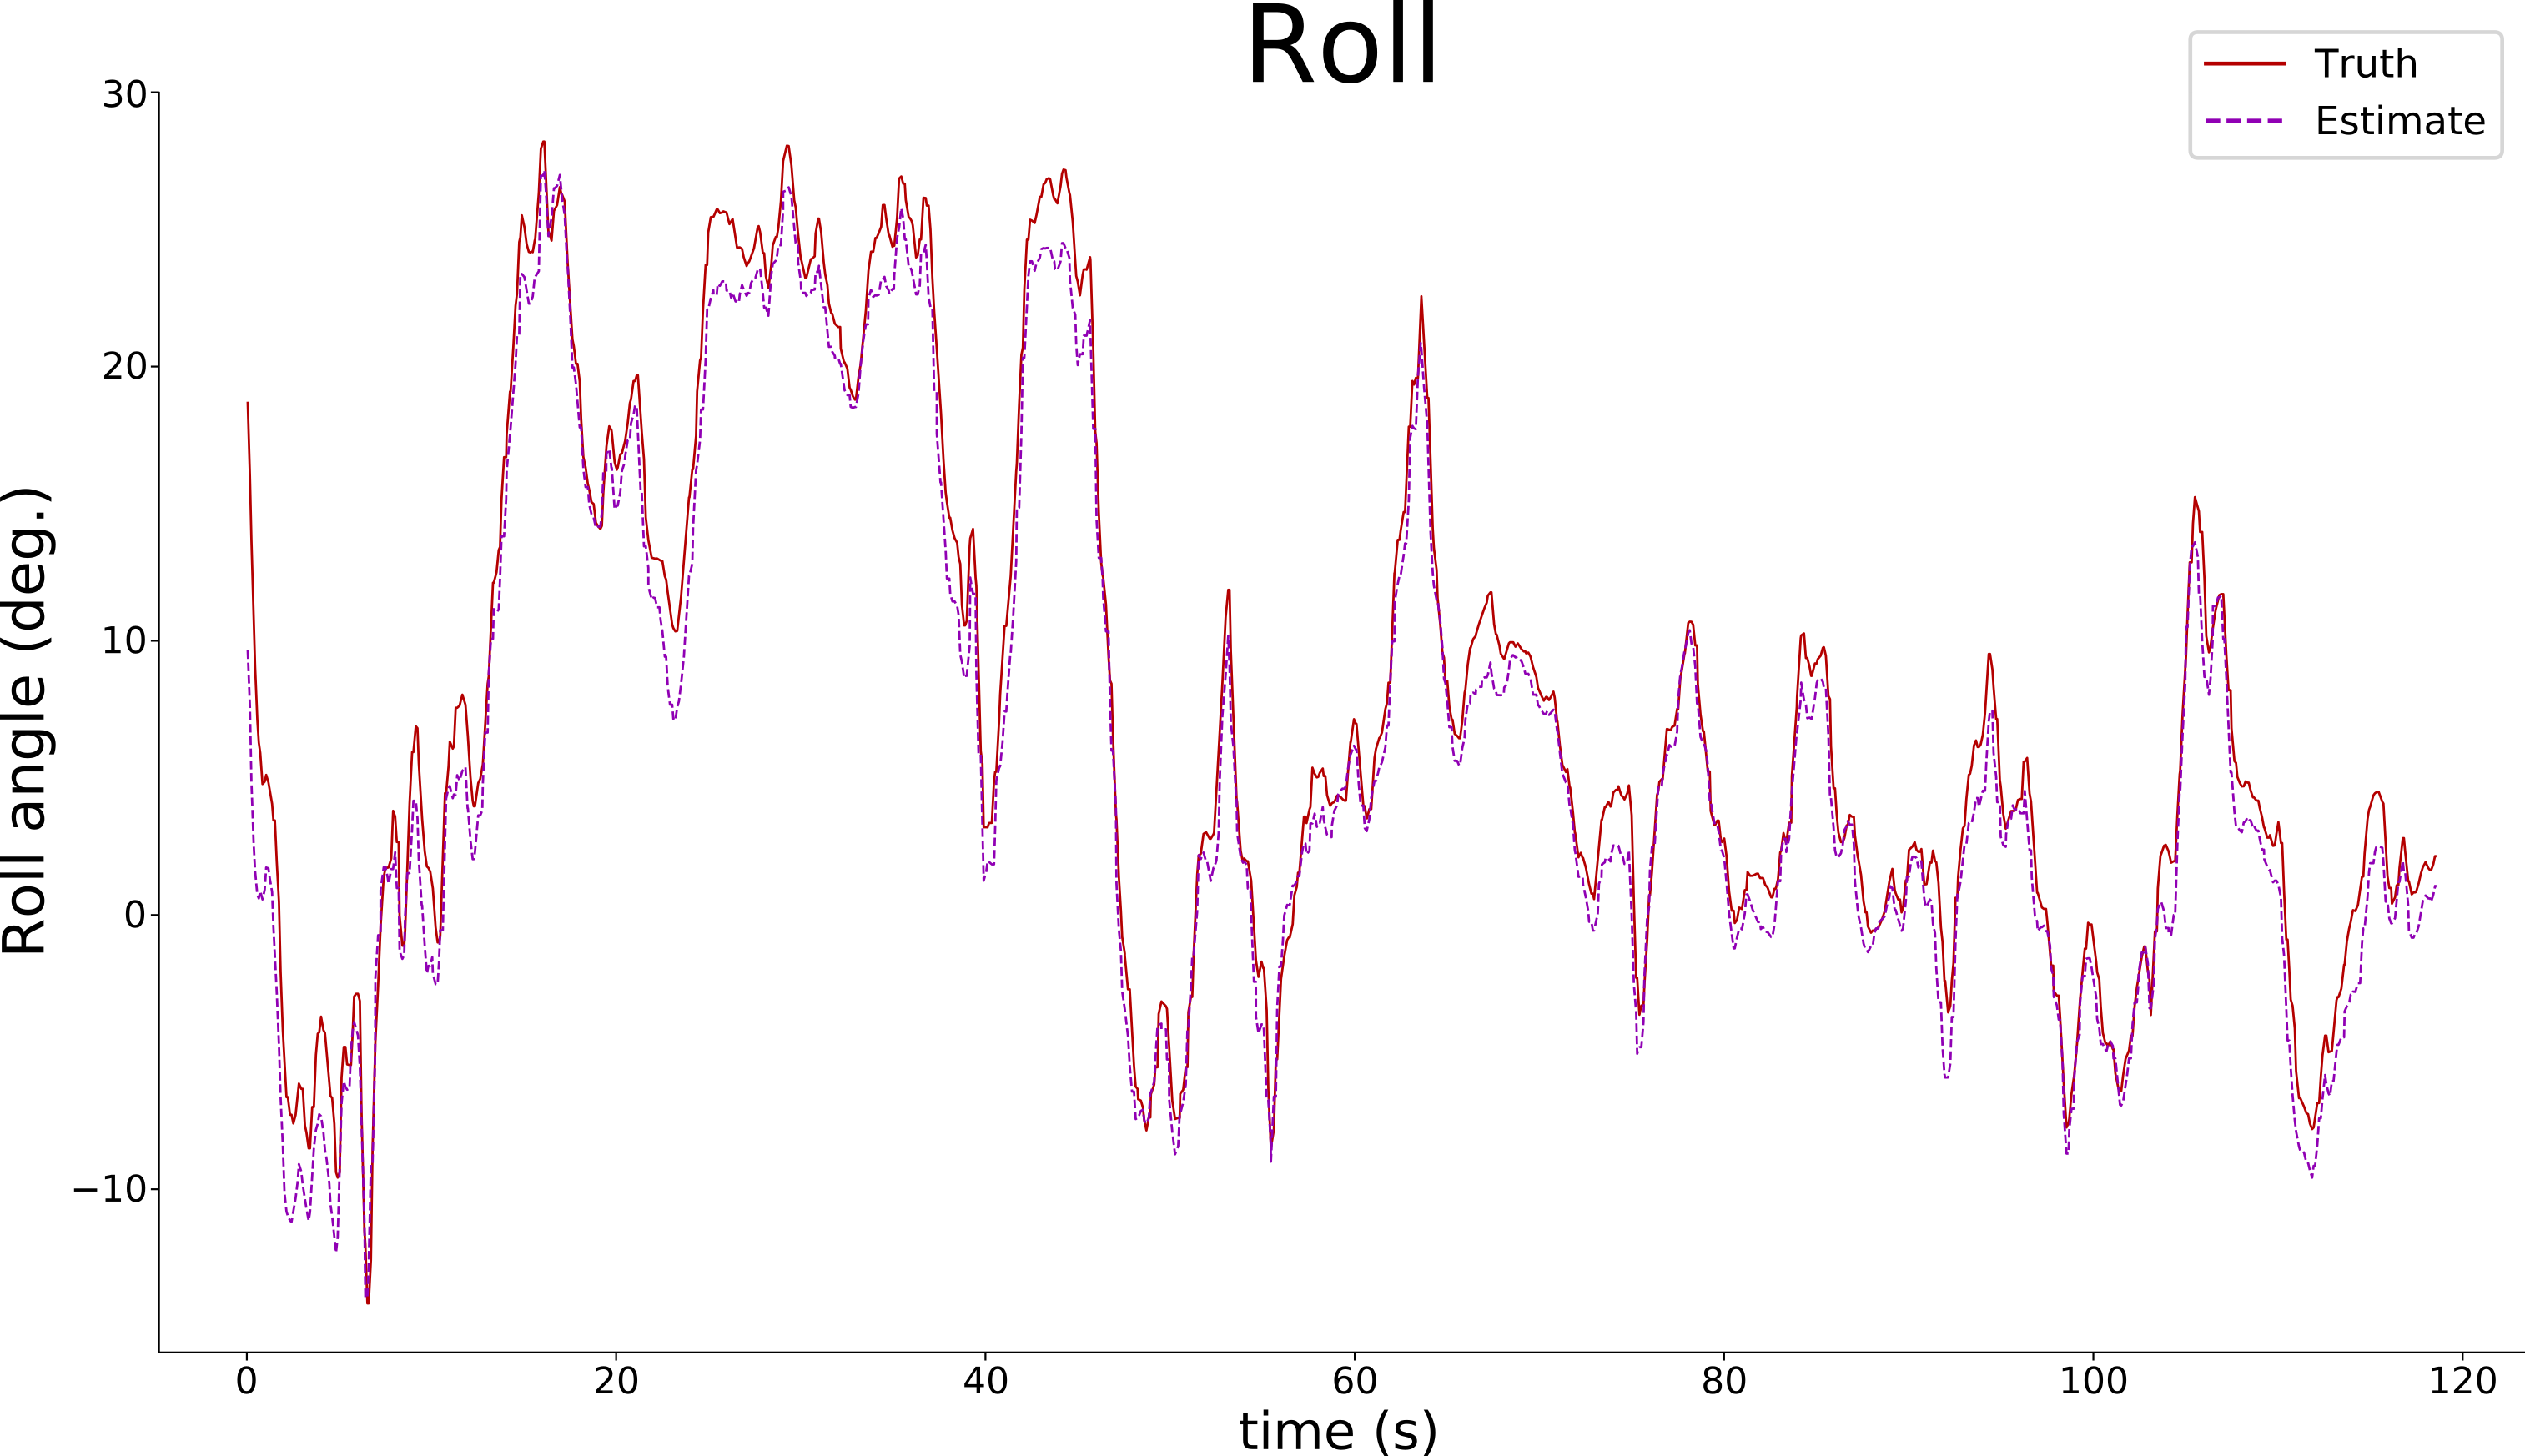
\includegraphics[width=\columnwidth]{figures/hardware_roll_plot}
	\caption{Plot of roll estimate during a hardware flight test.}
	\label{fig:roll_plot}
\end{figure}

\begin{figure}[hbt]
	\centering
	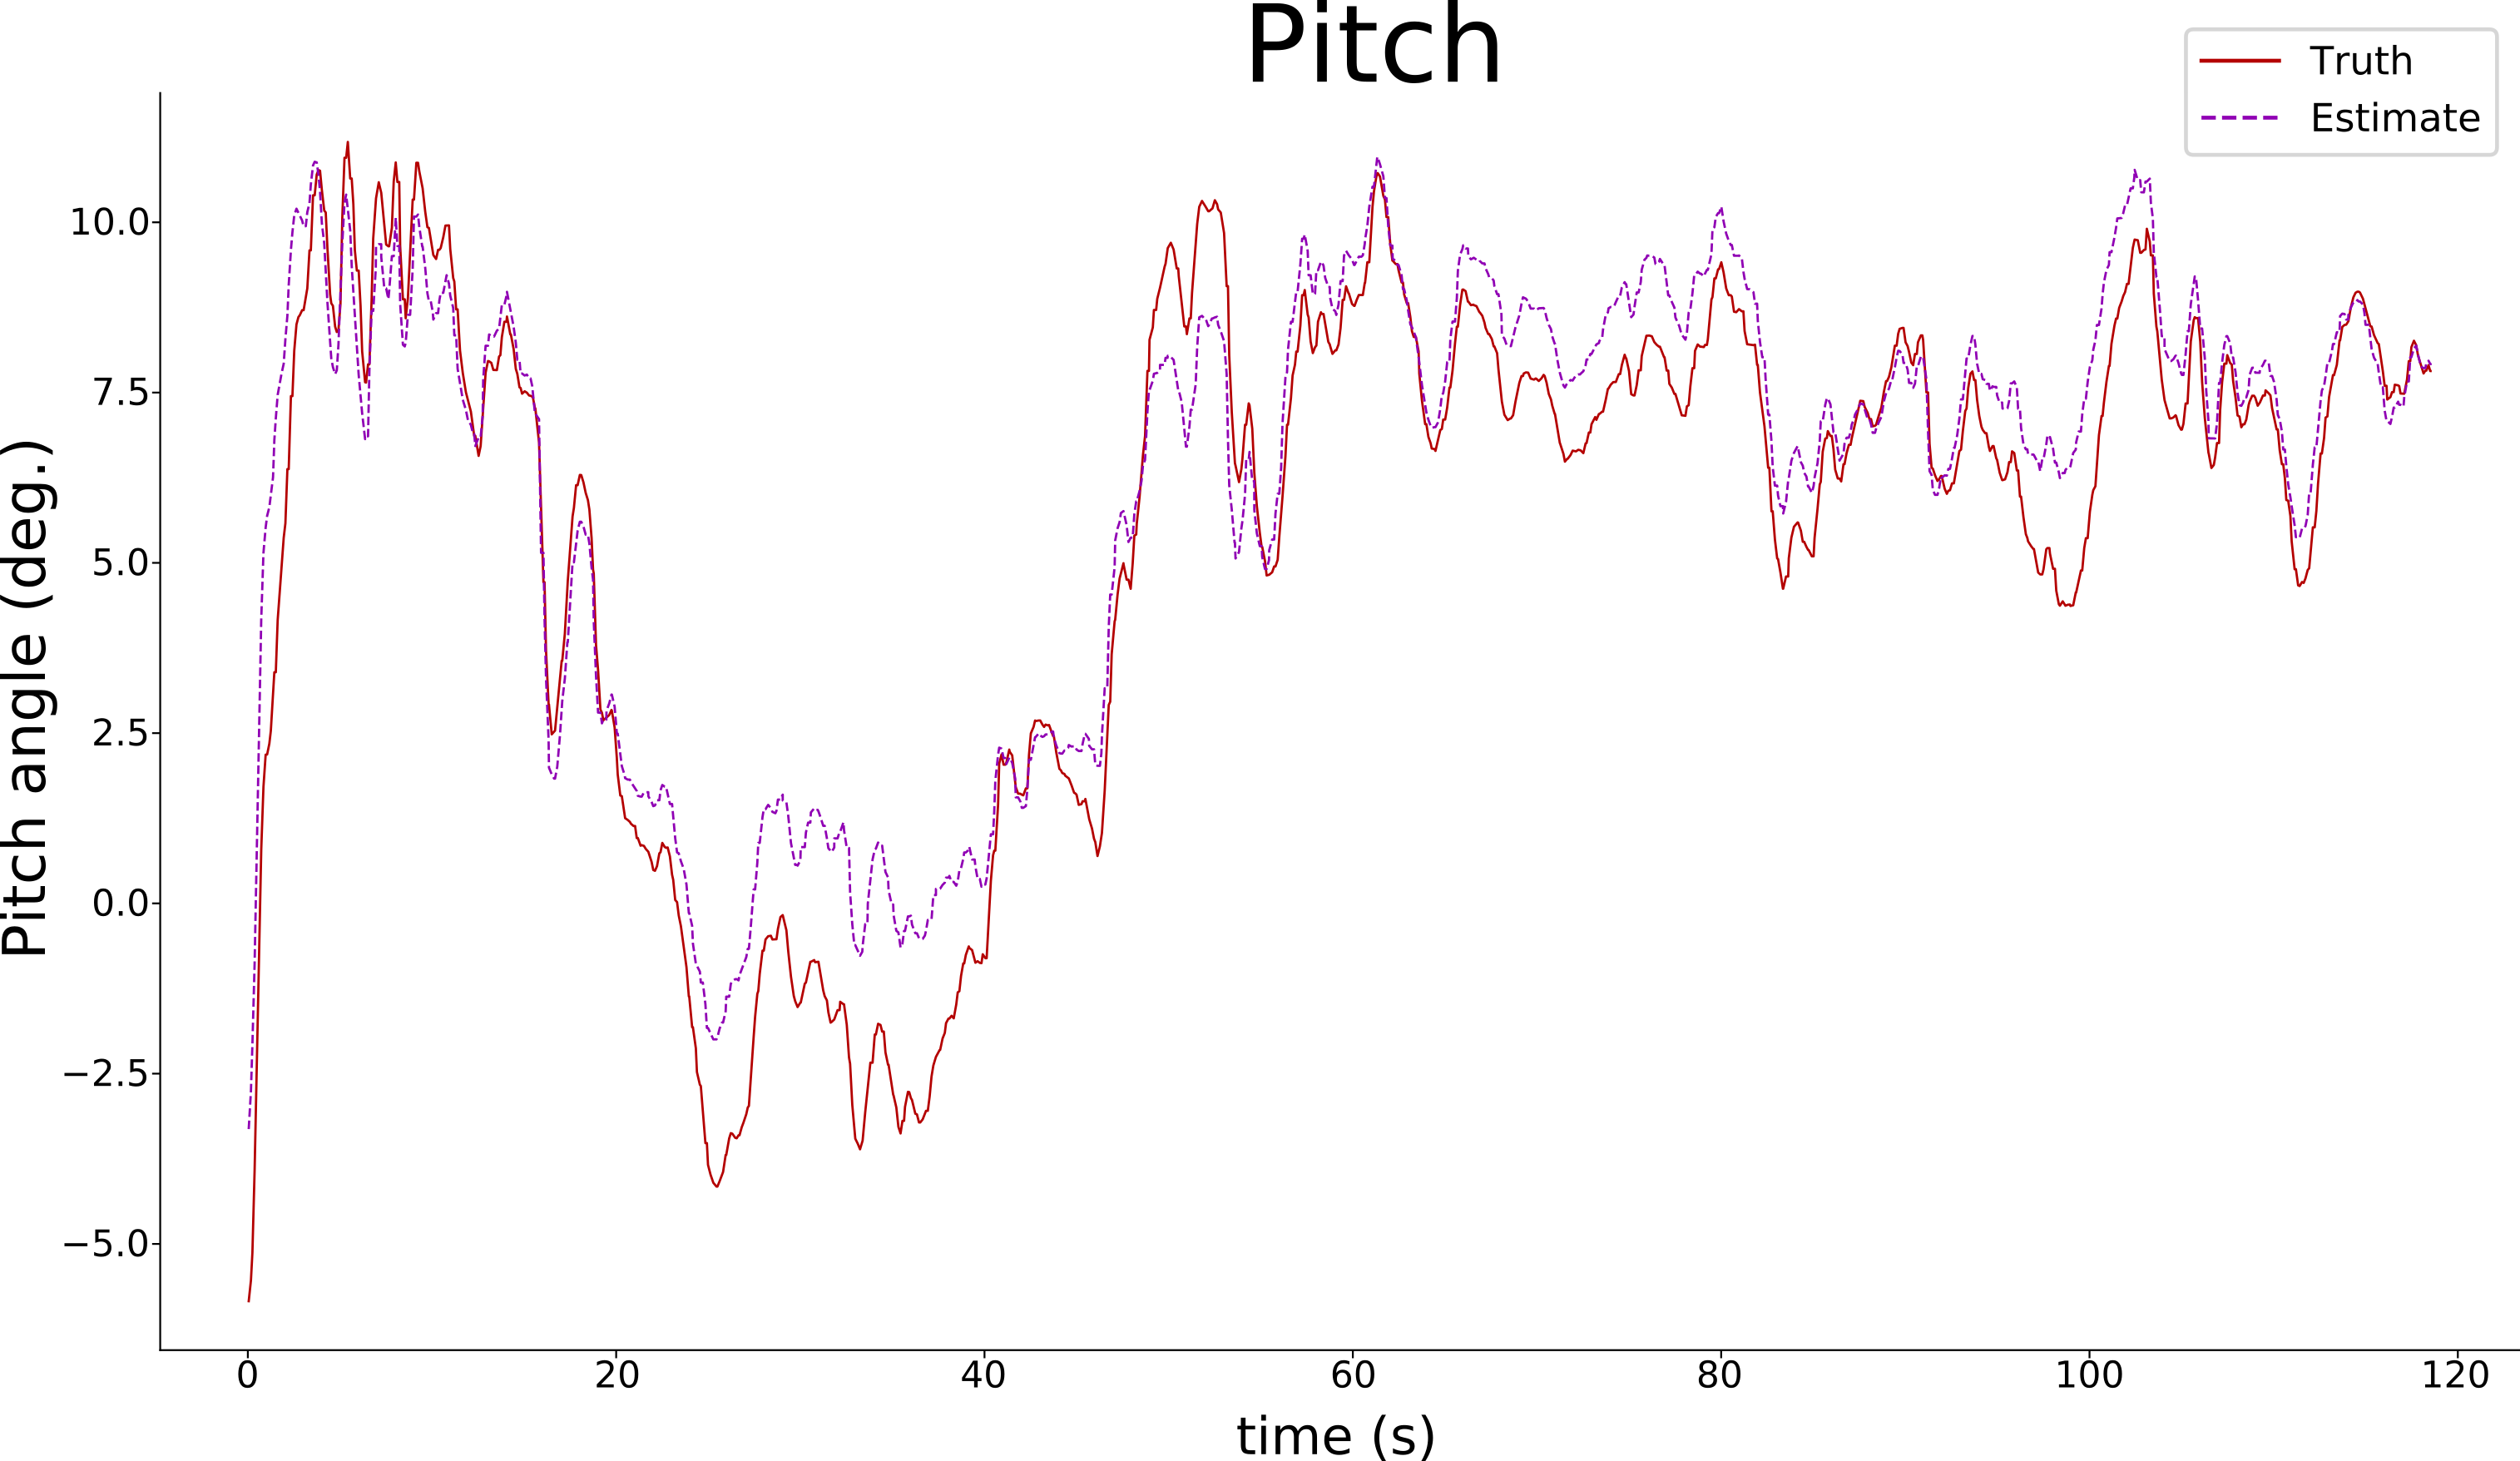
\includegraphics[width=\columnwidth]{figures/hardware_pitch_plot}
	\caption{Plot of pitch estimate during a hardware flight test.}
	\label{fig:pitch_plot}
\end{figure}

\begin{table}[hbt]
  \caption{Self-pose attitude estimation results}
	\label{tab:attitude_results}
	\resizebox{\columnwidth}{!}{%
	\begin{tabular}{c|l|l|}
	\cline{2-3}
	\multicolumn{1}{l|}{}                                                  & \multicolumn{1}{c|}{Roll} & \multicolumn{1}{c|}{Pitch} \\ \hline
	\multicolumn{1}{|c|}{Mean Squared Error (deg)} & 3.067                                             & 1.476                                              \\ \hline
	\multicolumn{1}{|c|}{Average Error (deg)}      & 1.277                                            & -0.655                                              \\ \hline
	\end{tabular}
	}
\end{table}

% Results and comparisons!
